
%(BEGIN_QUESTION)
% Copyright 2014, Tony R. Kuphaldt, released under the Creative Commons Attribution License (v 1.0)
% This means you may do almost anything with this work of mine, so long as you give me proper credit

Is this circuit's overall behavior capacitive or inductive?  In other words, from the perspective of the AC voltage source, does it ``appear'' as though a capacitor is being powered, or an inductor?

$$\includegraphics[width=15.5cm]{i01076x01.eps}$$

Now, suppose we take these same components and re-connect them in parallel rather than series.  Does this change the circuit's overall ``appearance'' to the source?  Does the source now ``see'' an equivalent capacitor or an equivalent inductor?  Explain your answer.

$$\includegraphics[width=15.5cm]{i01076x02.eps}$$

\vskip 20pt \vbox{\hrule \hbox{\strut \vrule{} {\bf Suggestions for Socratic discussion} \vrule} \hrule}

\begin{itemize}
\item{} Which component ``dominates'' the behavior of a series LC circuit, the one with the least reactance or the one with the greatest reactance?  
\item{} Which component ``dominates'' the behavior of a parallel LC circuit, the one with the least reactance or the one with the greatest reactance?
\end{itemize}

\underbar{file i01076}
%(END_QUESTION)





%(BEGIN_ANSWER)

The first (series) circuit's behavior is predominantly {\it inductive}, with 961.3 ohms of inductive reactance overshadowing 884.2 ohms of capacitive reactance, for a total circuit impedance of 77.13 ohms $\angle$ +90$^{o}$ (polar form) or 0 + j77.13 ohms (rectangular form).  

\vskip 10pt

The second (parallel) circuit's behavior is {\it capacitive}, with 1.131 millisiemens of capacitive susceptance overshadowing 1.040 millisiemens of inductive susceptance, for a total circuit admittance of 90.74 microsiemens $\angle$ +90$^{o}$.  This translates into a total circuit impedance of 11.02 k$\Omega$ $\angle$ $-90^{o}$, the negative phase angle clearly indicating this to be a predominantly capacitive circuit.

%(END_ANSWER)





%(BEGIN_NOTES)

As usual, the real point of this question is to get students to think about the analytical procedure(s) they use, and to engage their minds in problem-solving behavior.  Ask them {\it why} they think the circuits behave inductively or capacitively.

\vskip 10pt

Students often have difficulty formulating a method of solution: determining what steps to take to get from the given conditions to a final answer.  While it is helpful at first for you (the instructor) to show them, it is bad for you to show them too often, lest they stop thinking for themselves and merely follow your lead.  A teaching technique I have found very helpful is to have students come up to the board (alone or in teams) in front of class to write their problem-solving strategies for all the others to see.  They don't have to actually do the math, but rather outline the steps they would take, in the order they would take them.  The following is a sample of a written problem-solving strategy for analyzing a series resistive-reactive AC circuit:

\vskip 10pt

\goodbreak

{\bf Step 1:} Calculate all reactances ($X$).

{\bf Step 2:} Draw an impedance triangle ($Z$ ; $R$ ; $X$), solving for $Z$

{\bf Step 3:} Calculate circuit current using Ohm's Law: $I = {V \over Z}$

{\bf Step 4:} Calculate series voltage drops using Ohm's Law: $V = {I Z}$

{\bf Step 5:} Check work by drawing a voltage triangle ($V_{total}$ ; $V_1$ ; $V_2$), solving for $V_{total}$

\vskip 10pt

By having students outline their problem-solving strategies, everyone gets an opportunity to see multiple methods of solution, and you (the instructor) get to see how (and if!) your students are thinking.  An especially good point to emphasize in these ``open thinking'' activities is how to check your work to see if any mistakes were made.

%INDEX% Electronics review: AC reactance and impedance

%(END_NOTES)


